\chapter{Foutopsporing in JavaScript}

Een belangrijk onderdeel van programmeren is het opsporen van fouten in code. Soms gaat de geschreven code een uitkomst berekenen die niet correct is, en soms gebeurt er helemaal niets omdat de code een fout bevat (een syntactische fout, of het gebruik van een niet-gedefinieerde methode bijvoorbeeld). In het laatste geval laat de web browser standaard geen foutmelding zien, omdat de ontwikkelaars van de browsers er van uit gaan dat gewone gebruikers niet veel kunnen met foutmeldingen van scripts. Voor ons is dit gedrag van de browser natuurlijk onhandig, aangezien wij graag w\'el op de hoogte gesteld worden van fouten in onze scriptjes.

Gelukkig kunnen browsers deze foutmeldingen wel geven, maar je moet deze functionaliteit eerst aanzetten. Open de HTML-pagina met de code in waar je een fout wil opsporen, en open dan de `developer tools' van je browser. Waar je op moet klikken (of welke toetsencombinatie je moet gebruiken) hangt af van je browser.

\paragraph{Chrome}

Druk \key{CTRL} + \key{SHIFT} + \key{J} om Developer Tools te openen en het `Console'-tabblad te kiezen
Alternatieve methode: Druk \key{F12} om Developer Tools te openen.

\paragraph{Safari}

Druk \key{CTRL} + \key{ALT} + \key{I} om 'Web Inspector' te openen.

\paragraph{Internet Explorer 9+}

Druk \key{F12} om Developer Tools te openen. Klik daarna op het 'Script'-tabblad

\paragraph{Firefox}

Druk \key{CTRL} + \key{SHIFT} + \key{K} om `Web console' te openen, of druk F12 om Firebug te openen (indien dit ge\"installeerd is - aangeraden!). Klik daarna op het 'Console'-tabblad

\paragraph{Opera}

Druk \key{CTRL} + \key{SHIFT} + \key{I} om 'Dragonfly' te openen. Klik daarna op het `Console'-tabblad

\section{Debuggen}

Indien je een syntactische fout gemaakt hebt in je code, zal de browser je onmiddellijk aangeven waar de fout gemaakt is en wat hij denkt dat er fout is. Stel dat we bijvoorbeeld een kort stukje code schrijven waar we een sluitende accolade vergeten zijn, dan krijg je de foutmelding uit Figuur~\ref{fig:debug1}.

\begin{figure}
\centering
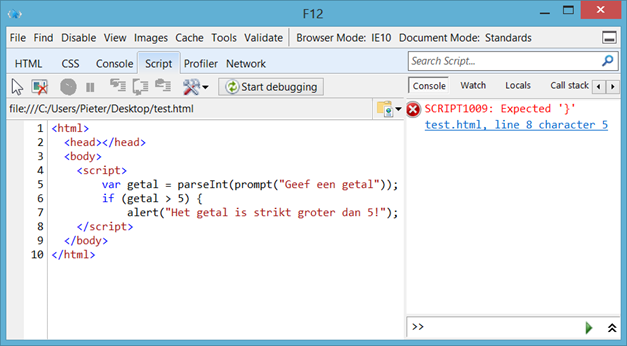
\includegraphics[scale=0.8]{Debuggen/debug1.png}
\caption{Een scriptfout in het debugvenster}\label{fig:debug1}
\end{figure}

De browser zegt dus wat er fout is (``Expected `\}'") en geeft ook aan op welke lijn hij de fout opmerkte. Alhoewel de foutmeldingen vaak zeer precies en correct zijn, kan het soms toch voorvallen dat de beschrijving een beetje misleidend is of dat het lijnnummer niet overeenkomt met de feitelijke locatie van de fout. Deze foutopsporingsmodus moet je dus vooral zien als handig hulpmiddel, en dus niet als een orakel dat altijd een 100\%-correcte beschrijving van het probleem geeft.

Indien je code schrijft maar er niets gebeurt wanneer je de pagina in je browser laadt, dan duidt dit bijna altijd op een syntactische fout in je code. In dit geval start je dus best deze debugger op, en waarschijnlijk krijg je direct een goede beschrijving van waar de fout ligt.
Soms gaat je code wel degelijk iets berekenen maar is het resultaat helaas niet wat er verwacht werd. In zulke gevallen is het vaak handig om stapsgewijs door de code te gaan om zo te zien waar de fout precies aan ligt. Ook deze manier van fouten opsporen wordt ondersteund door de debugger van onze browser. De precieze manier om stapsgewijs door de code te gaan hangt af van browser tot browser. In deze tekst zal getoond worden hoe dit werkt in Internet Explorer, maar het proces is analoog voor andere browsers.

Stel dat je de volgende code hebt geschreven om de som van de cijfers van een getal te berekenen:

\begin{minipage}{\linewidth}
\lstset{language=JavaScript,basicstyle=\small}
\begin{lstlisting}
function berekenSomCijfers(getal) {
    var som = 0;
    while (getal > 0) {
        var r = getal % 10;
        som = som + r;
        getal = getal / 10;
    }
    return som;
}
var res = berekenSomCijfers(18493);
alert("De som van de cijfers is " + res);
\end{lstlisting}
\end{minipage}

Helaas bevat deze code een fout; het antwoord dat de browser toont is `27.77777777777774' wat natuurlijk niet juist is. Op het eerste zicht ziet de code er echter juist uit, dus we zullen gebruik moeten maken van de debugger in de browser om de fout op te sporen.

Open de developer tools (door op \key{F12} te drukken) en ga naar het Script-tabblad. Je ziet nu de code staan die je geprogrammeerd hebt. Het eerste wat we nu moeten doen is een breakpoint instellen. Dit is een bepaald punt in de code waar de debugger de uitvoering van het script zal pauzeren en de optie zal geven aan de programmeur om te kijken wat op dat moment de waardes zijn van alle variabelen. We stellen een breakpoint in door te klikken in de marge voor de lijnnummers, waardoor er een rood bolletje tevoorschijn komt. Figuur~\ref{fig:debug2} toont een breakpoint op lijn 8 (gemarkeerd met een `1'). Van zodra het breakpoint gezet is, moeten we aan de browser zeggen dat we de foutopsporing willen starten door op de knop 'start debugging' (gemarkeerd met een `2') te klikken. Nu gaan we terug naar ons browservenster waar de pagina in geladen is, en we drukken op `vernieuwen'.

\begin{figure}
\centering
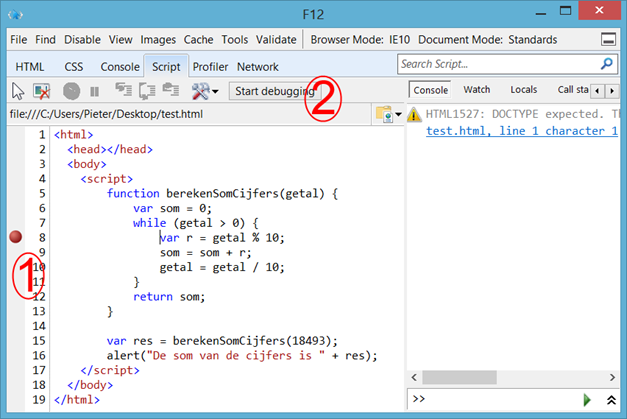
\includegraphics[scale=0.8]{Debuggen/debug2.png}
\caption{Starten met het debuggen}\label{fig:debug2}
\end{figure}

Op het moment dat we op `vernieuwen' klikken, zal de pagina opnieuw geopend worden en wordt het scriptje dus uitgevoerd. Van zodra de browser bij het breakpoint komt dat we ingesteld hadden zal hij de uitvoering van het scriptje stoppen en vragen aan de gebruiker hoe die verder wil gaan. We krijgen het scherm van Figuur~\ref{fig:debug3} te zien:

\begin{figure}
\centering
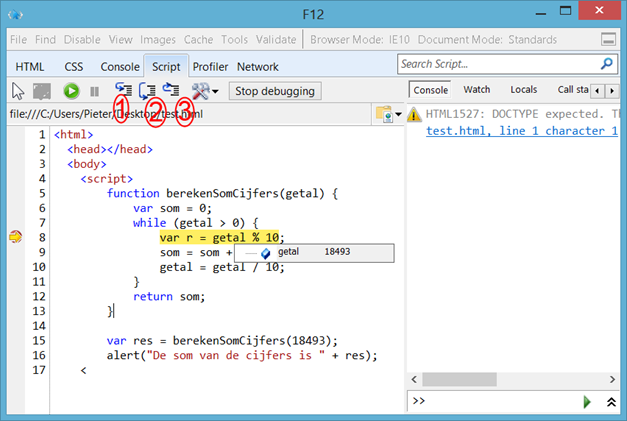
\includegraphics[scale=0.8]{Debuggen/debug3.png}
\caption{De debugopties}\label{fig:debug3}
\end{figure}

De plaats waarop de uitvoering gepauzeerd is, is gemarkeerd met een gele achtergrond. Merk op dat de uitvoering gestopt wordt voordat de lijn met het breakpoint uitgevoerd is! Op dit moment kunnen we kijken wat de waarde is van de verschillende variabelen in onze code door gewoon met de muis er over te gaan staan. Als we met de muis op `getal' gaan staan, dan krijgen we te zien dat de waarde van getal op 18493 staat, wat inderdaad de waarde is die we verwachten.
De knoppen die net boven de code staan (gemarkeerd met de cijfers 1, 2 en 3) laten ons toe om nu stapsgewijs door de code te gaan om te kijken wat er precies misloopt. De knop die met een `2' gemarkeerd is, is de `Step Over'-knop (\key{F10}). Als we hier op klikken, dan gaat de browser de lijn waar de uitvoering momenteel gepauzeerd is uitvoeren, en terug stoppen voordat de volgende lijn uitgevoerd wordt. In bovenstaand voorbeeld zou de lijn var r = getal \% 10; uitgevoerd worden en zal de browser terug stoppen voor lijn 9. Op dit punt kunnen we dus weer de staat van de variabelen bekijken en zien of alles nog is zoals we verwachten.

De knop die met `1' gemarkeerd is, is de `Step Into'-knop (\key{F11}). Indien de lijn waar de browser op gepauzeerd is een functie is, en we drukken op deze knop, dan gaat de browser springen naar de functie  die opgeroepen wordt en gaat die daar op de eerste lijn stilstaan. Merk op dat indien we hier op de `Step Over'-knop zouden gedrukt hebben, dat de browser de volledige functie gaat uitvoeren en dan pas terug de code pauzeren.

De knop die met `3' gemarkeerd is, is de `Step Out'-knop (\key{SHIFT} + \key{F11}). Indien de uitvoering gepauzeerd is in een functie en we drukken op deze knop, zal de browser de rest van de functie uitvoeren en terug pauzeren op de plaats waar de functie opgeroepen werd.

Door gebruik te maken van deze drie knoppen kunnen we dus gemakkelijk stapsgewijs door onze code lopen. Zo kunnen we al vlug de oorzaak vinden van de fout. We zien dat na de lijn getal = getal / 10; de waarde van getal niet correct is. Om juist te werken zou na deze deling alle getallen achter de komma moeten wegvallen, maar zoals we in onze debugger kunnen zien is dit niet het geval. Dit is dan ook de reden van onze foutieve uitkomst.

\begin{figure}
\centering
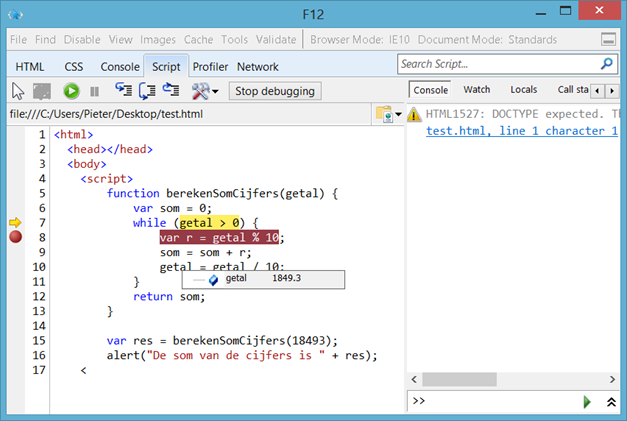
\includegraphics[scale=0.8]{Debuggen/debug4.png}
\caption{De debugger in actie}\label{fig:debug4}
\end{figure} 